\chapter*{M5: Multicore}{Section Author: Sahil Gupta}
\addcontentsline{toc}{chapter}{M5: Multicore}
\section{Architecture Overview}

For multicore, our architecture is quite simple and straightforward. Cores are brought up by
invoking the correct PSCI functions through the kernel (the same method is used for shutdown, reset,
and reboot, as discussed later). Communication between cores for this specific milestone is handled
through the \co{initial_urpc} struct, which lives in main memory. The relevant code for this milestone
can be found in the following files:
\begin{itemize}
    \itemsep-0.5em
    \item \co{usr/init/coreboot.c}
    \item \co{usr/init/coreboot.h}
    \item \co{usr/init/main.c}
    \item \co{usr/init/mem_alloc.c}
    \item \co{usr/init/mem_alloc.h}
\end{itemize}
Bonus work is discussed in the Suspend, Resume, Shutdown, and Reboot section.
Below is a simple diagram outlining the process of booting the different cores and communicating with them.

\begin{figure}[H]
    \centering
    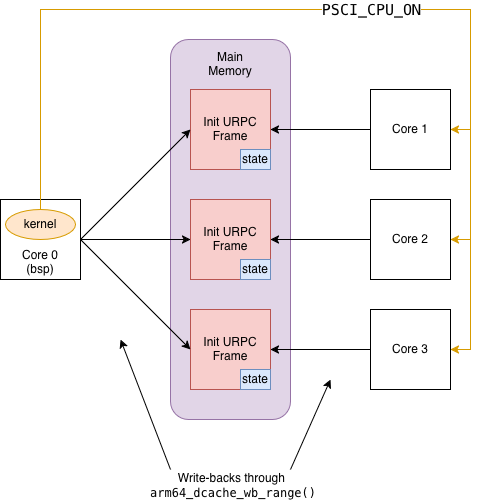
\includegraphics[width=0.5\textwidth]{images/m5_arch.drawio(1).png}
    \caption{Multicore Architecture}
    \label{fig:m5arch}
\end{figure}

\subsection{Initial URPC Frame}

Before discussing any of the code written for this milestone, or any of the functionality, we need to discuss the
core struct for communicating with the booted cores, which contains some new fields.

\begin{lstlisting}
struct initial_urpc {
    genpaddr_t           bootinfo_frame_base;
    gensize_t            bootinfo_frame_bytes;
    genpaddr_t           mmstr_frame_base;
    gensize_t            mmstr_frame_bytes;
    genpaddr_t           ram_base;
    gensize_t            ram_bytes;
    volatile corestate_t state;
    uint32_t             active_cores_mask;
    struct {
        genpaddr_t base;
        gensize_t  bytes;
    } peer_rings[COREBOOT_MAX_CORES];
};
\end{lstlisting}
The fields \co{active_cores_mask} and \co{peer_rings} are used for User-Level Message Passing and can be ignored for now.
The rest of the fields are used to boot up different cores, pass memory from the BSP core, and communicate the state of
the booted core.

\begin{description}
    \setlength{\itemsep}{2pt}
    \item[\co{bootinfo_frame_base}, \co{bootinfo_frame_bytes}] Used to pass the booted core
        information about the \co{bootinfo} struct so it can be forged on the booted core.
        The \co{bootinfo} struct contains memory layout information crucial for the core to
        allocate memory.
    \item[\co{mmstr_frame_base}, \co{mmstr_frame_bytes}] Passed to the booted core to forge
        the relevant capability, used to discover module names for processes spawned on that core.
    \item[\co{ram_base}, \co{ram_bytes}] A region of RAM donated from the BSP core to give the
        newly spawned core memory to work with.
    \item[\co{state}] A synchronization flag with several states, modifiable by either the BSP
        core or the spawned core to communicate boot progress.
\end{description}

\subsection{Booting Another Core}
Now we can talk about the process of spawning a new core. The following steps are executed by the
BSP core at startup, which invokes \co{coreboot_boot_core} on every core (we support booting
every core on the Toradex board).
\begin{enumerate}
    \itemsep-0.5em
    \item Allocate and fill in the Initial URPC frame, then flush it to main memory so the booted core can see it
    \item Locate the correct binaries for the CPU driver, boot driver, and the \co{init} program
    \item Load the relevant ELFs and relocate them
    \item Allocate a new KCB and fill in the relevant fields
    \item Call \co{invoke_monitor_spawn_core}, which in turn invokes \co{PSCI_CPU_ON} through the kernel to spawn the core
    \item Wait for the spawned core to signal it is ready
\end{enumerate}
On the spawned core, execution begins in the \co{app_main} function in \co{usr/init/main.c},
which forges the correct capabilities and signals readiness to the BSP core by setting the
\co{state} field.

\subsection{Multicore Memory Management}
Due to the design of Barrelfish, managing memory across multiple cores is non-trivial, as each
core must know what memory it is responsible for. In our design, the BSP core carves out a fixed
region of memory to hand over to the spawned core, using the \co{ram_}* fields of the
\co{initial_urpc} struct and \co{ram_alloc}. We fix the size of this region at 128 MiB which is large
enough for the new core to boot, but small enough not to starve the BSP core. We arrived at this
value through empirical testing, and note that other values may be more appropriate depending on
the multicore workload.

\subsection{Suspend, Resume, Shutdown, and Reboot}
In this milestone, we support the ability to suspend, resume, shutdown, and reboot a core (though
reboot is not fully functional), implemented primarily through the \co{initial_urpc} struct.
First, we need to revisit the \co{state} field. Its type is shown below:
\begin{lstlisting}
typedef enum corestate {
    CORE_STATE_UNKNOWN,
    CORE_STATE_OFF,
    CORE_STATE_RUNNING,
    CORE_STATE_SLEEPING,
} corestate_t;
\end{lstlisting}
When the BSP core spawns a new core, the field is initialized to \co{CORE_STATE_UNKNOWN} and
the newly spawned core then sets it to \co{CORE_STATE_RUNNING} once it is ready. This pattern
lets a remote core detect when its state needs to change based on a signal from another core.

\medskip\noindent
Suspend and shutdown are the simplest functions. Since equivalent PSCI functions exist, we create
monitor entry points into the kernel and invoke them directly. When the BSP core instructs a remote
core to suspend or shut down, it updates the \co{state} field in the URPC struct
(\co{CORE_STATE_SLEEPING} for suspend, \co{CORE_STATE_OFF} for shutdown). The remote core polls
this field in \co{app_main} and acts accordingly. This same signaling pattern is used for the
other lifecycle functions.

\medskip\noindent
For resume, there is no direct PSCI function. According to the PSCI specification, a suspended
core requires a wakeup event to resume. We use a Software Generated Interrupt (SGI) as the wakeup
event, implemented via a monitor syscall that invokes \co{gic_raise_softirq} on the suspended core
from the kernel.

\medskip\noindent
For reboot, we do not support a core rebooting itself and the only supported path is the BSP core
rebooting a remote core. We accomplish this by first signaling the remote core to shut down, then
invoking \co{coreboot_boot_core} on the same core ID.

\section{Development Process}

This milestone began with implementing the main functionality in \co{coreboot_boot_core} in
\co{usr/init/coreboot.c}, where we allocated all the necessary data structures and set up the
shared URPC frame. In this part, we also enabled booting all cores on the Toradex board by
modifying \co{usr/init/main.c}.

\medskip\noindent
We then implemented memory allocation on remote cores, which involved allocating a large chunk of
memory through \co{ram_alloc} and passing it through the URPC frame. We also needed a way to
initialize the allocator from a forged capability, which required us to implement
\co{initialize_ram_alloc_from_cap} in \co{usr/init/mem_alloc.c}.

\medskip\noindent
Finally, we implemented all the core lifecycle functions and wrote sample test cases to demonstrate
the functionality.